\atsp
\begin{frame}{\ft{Configuring the Data Set Application}}
\section{Group 1: Configuring the Data Set Application}

\begin{annotatedFigure}{0pt}{0pt}{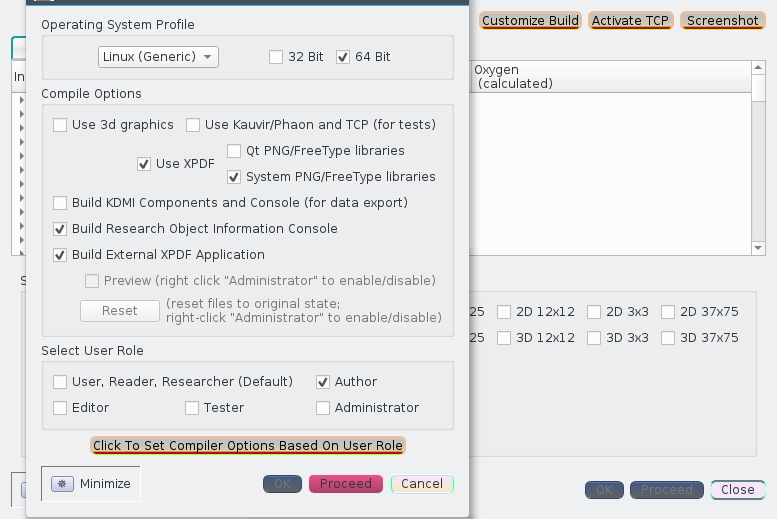
\includegraphics[scale=1.5]{texs/config.png}}
            
  \node [text width=8.1cm,align=justify,fill=logoCyan!20, draw=logoBlue, 
  draw opacity=0.5,line width=1mm, fill opacity=0.9]
   at (0.79,0.72){\textbf{Using Qt Creator, the Dataset Creator 
   will automatically launch the main Dataset \mbox{Application} 
   with every feature needed in order to \mbox{visualize} 
   and explore the data.  In 
   addition, the data set includes several 
   configurations allowing users to incorporate more specialized 
   or complex features, such as XPDF, test suites, and 
   data export code.  Users can fine-tune which additional 
   features they wish to utilize --- via a separate dialog box 
   \mbox{(\circled{1} and \circled{2})} --- to create a customized build of the 
   main Dataset Application and supplemental executables.}};

  \annotatedFigureBox{0.61,0.93}{0.75,0.982}{1}{0.75,0.922}%
            \annotatedFigureBox{0.033,0.12}{0.58,0.97}{2}{0.58,0.97}%            
      %      \annotatedFigureBox{0.222,0.284}{0.3743,0.4934}{B}{0.3743,0.4934}%tr
      %      \annotatedFigureBox{0.555,0.784}{0.6815,0.874}{C}{0.555,0.784}%bl
      %      \annotatedFigureBox{0.557,0.322}{0.8985,0.5269}{D}{0.8985,0.5269}%tr
    \node [text width=7cm,align=justify,fill=logoCyan!20, draw=logoBlue, 
    draw opacity=0.5,line width=1mm, fill opacity=0.9]
     at (0.778,0.3){\textbf{The Dataset Creator 
     also recognizes distinct ``roles" (\circled{2}), including 
     general readers, authors, those who double-check the 
     main Dataset Application via a test suite, and those 
     who design the test suite and write dataset code overall 
     (dubbed ``Administrators").}};
  
   \annotatedFigureBox{0.05,0.16}{0.57,0.35}{2}{0.57,0.35}
        
      
  
        \end{annotatedFigure}

   %     \caption{Expanded Sample (A)}
    %    \label{fig:teaser}

    \end{frame}


